\subsubsection{User}
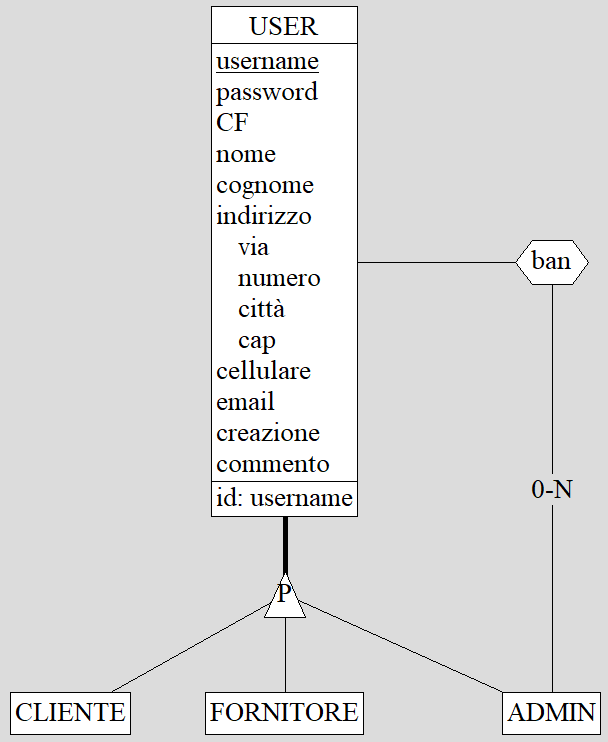
\includegraphics[width=0.95\columnwidth]{User.png}\\
I tre tipi di account che potranno essere creati, \textbf{CLIENTE}, \textbf{FORNITORE}, \textbf{ADMIN},  saranno sottocategorie di \textbf{USER}. Data la possibilità che una persona crei più di un account, ad esempio un fornitore vuole anche essere un cliente, l'identificazione avverrà tramite \textbf{username} e non il \textbf{CF}(codice fiscale).



\subsubsection{Ente}
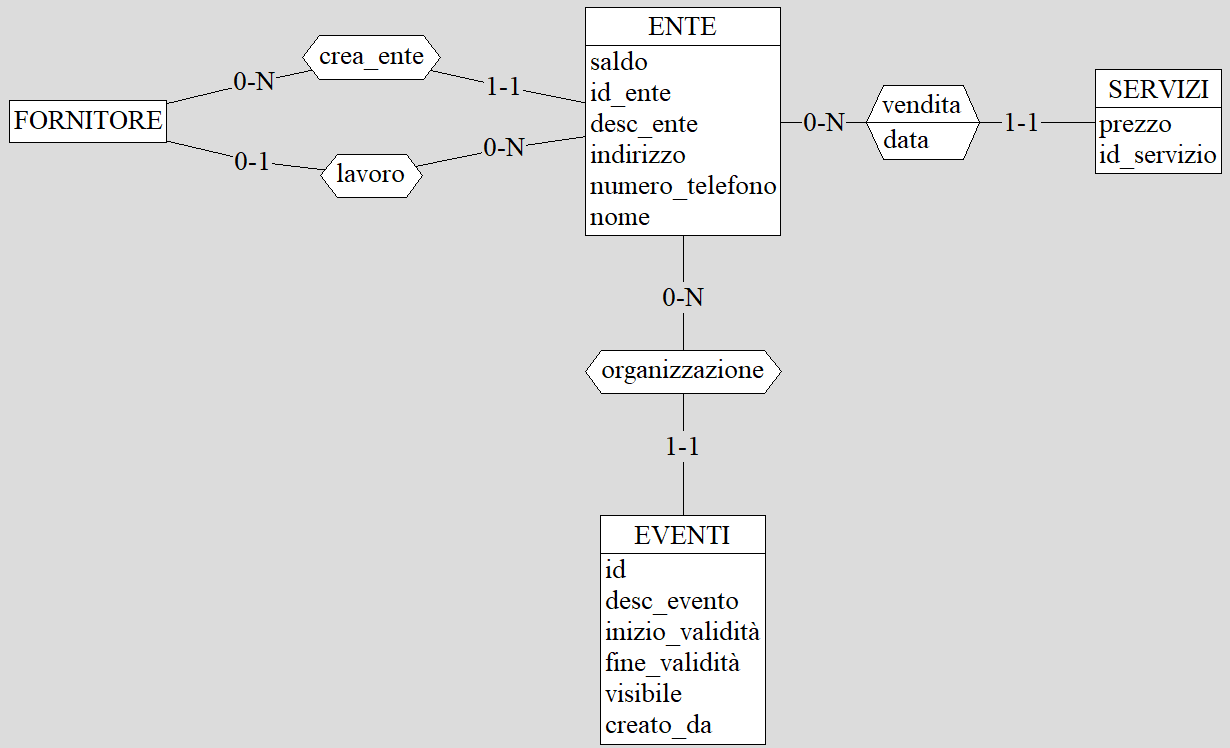
\includegraphics[width=0.95\columnwidth]{images/Ente.png} \\
L'ente è l'organizzazione che vende i servizi e organizza gli eventi. 
I fornitori possono lavorare per più di un ente.
Gli enti creano post e decidono quando pubblicarli/renderli pubblici. 


\subsubsection{Eventi}
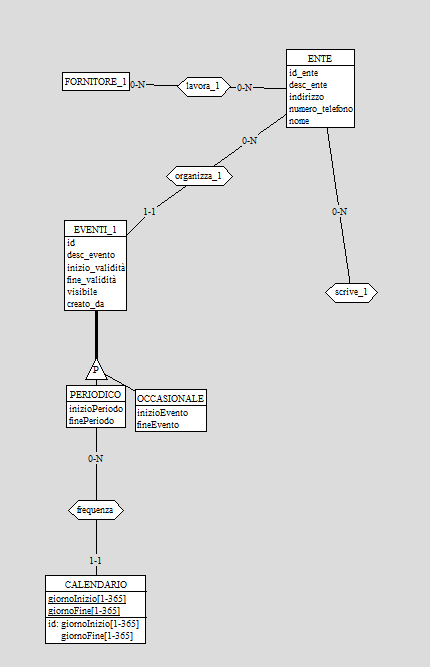
\includegraphics[width=0.95\columnwidth]{images/Eventi.png} \\
I servizi sono gli avvenimenti gratuito accessibili con o senza prenotazione.
Sono organizzati dagli enti, un ente può organizzare più eventi ma un evento appartiene ad un solo ente.
Un evento può accadere in modalità periodica (ad esempio eventi a tema natalizio) oppure in modo occasionale (ad esempio inaugurazione di una nuova gelateria in centro)
\subsubsection{CityCard}
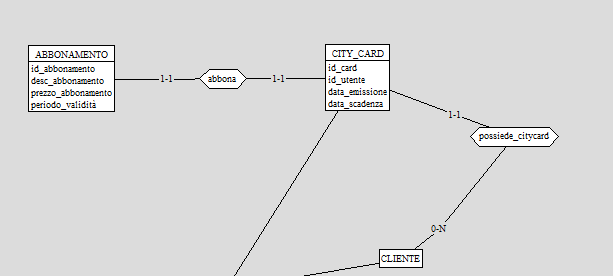
\includegraphics[width=0.95\columnwidth]{images/CityCard.png} \\
Ogni cliente può ottenere una CityCard che  permetterà l'utilizzo gratuito dei mezzi pubblici e la prenotazione e l'acquisto di servizi forniti dagli enti comunali e regionali. Per attivare la CityCard sarà necessario sottoscrivere ad un abbonamento a scelta tra tre diverse durate, dalla scelta fatta varierà la validità e gli sconti offerti  per l'acquisto dei servizi.
\subsubsection{Carta di credito} 
Ogni cliente, tramite la carta di credito, potrà acquistare la city card e pagare gli enti che forniscono i servizi
\subsubsection{Sezione delle news}
Una volta avuto accesso al portale ci sarà una sezione dedicata alle notizie relative ad eventi o servizi.
L'ente potrà creare un post in cui pubblicizza i servizi offerti o un'attività l'evento che sta organizzando
\subsubsection{Abbonamento}
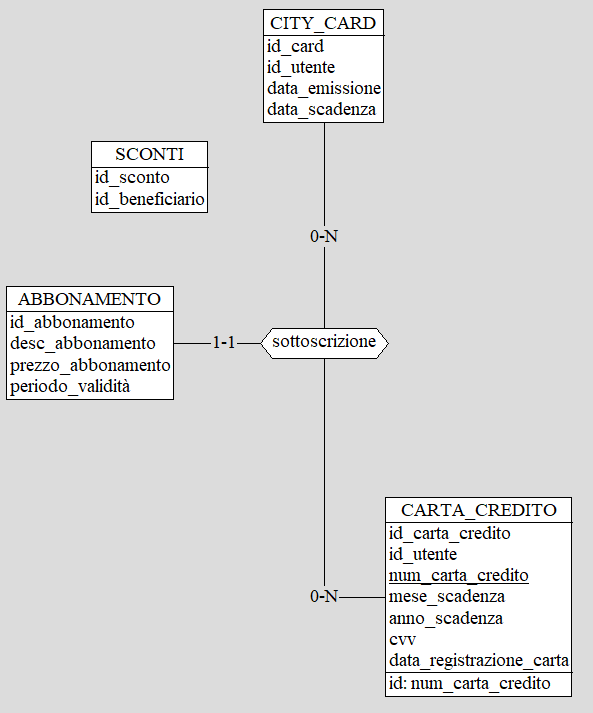
\includegraphics[width=0.95\columnwidth]{images/abbonamento.png}\\
L'abbonamento è lo strumento che permette l'attivazione della city card e, di conseguenza, l'acquisto di servizi. Ogni abbonamento ha una sua tipologia che l'utente potrà scegliere di acquistare. A prescindere dalla tipologia ogni abbonamento ha un suo prezzo e un periodo di validità.
\subsubsection{Sconti}
Lo sconto viene applicato in base ad alcune variabili: \\
    - età del cliente (se è sopra ai 65 anni di età) \\
    - se si è formato un gruppo si avrà una riduzione del servizio \\
Lo sconto si caratterizza per la percentuale di riduzione.